\documentclass[border={0cm 0.5cm 0.5cm 0.5cm}]{standalone}

\usepackage{amssymb}
\usepackage{amsmath}
\usepackage{wasysym}	%for \eighthnote
\usepackage{tikz}

%Music on a three-dimensional lattice (schematic representation)
%Wishart, Trevor. (1996). On Sonic Art. Amsterdam: Harwood Academic Publishers, p. 26 (fig. 2.4b)

\begin{document}
	
	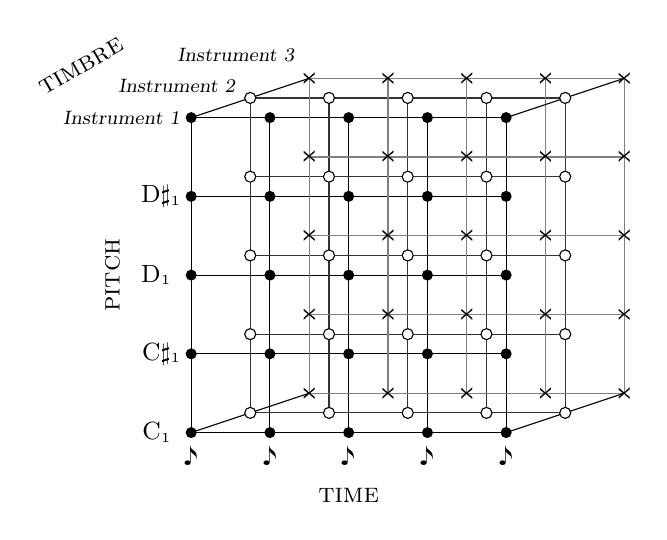
\begin{tikzpicture}	
	%GRIDS
	\draw (0,0) grid (4,4);
	\draw[black!80,xshift=0.75cm,yshift=0.25cm] (0,0) grid (4,4);
	\draw[gray,xshift=1.5cm,yshift=0.5cm] (0,0) grid (4,4);
		\draw (0,0)--(1.5,0.5);		\draw (0,4)--(1.5,4.5);
		\draw (4,0)--(5.5,0.5);		\draw (4,4)--(5.5,4.5);
	
	%DOTS
	\foreach \y in {0,...,4}{
	\node[align=center,below] at (\y,-0.05) {\eighthnote};
	\foreach \x in {0,...,4}{
		\fill (\x,\y) circle (2pt);
		\filldraw[fill=white,draw=black] (0.75+\x,0.25+\y) circle (2pt);
		\node at (1.5+\x,0.5+\y) {\rotatebox{90}{\sffamily\small x}};	
		} %end inner loop
	} %end outer loop
	
	%LABELS
	%\node[align=center] at (-1,2) {\textsc{p}\\[-2mm]\textsc{i}\\[-2mm]\textsc{t}\\[-2mm]\textsc{c}\\[-2mm]\textsc{h}};
	\node at (-1,2) 	 {\rotatebox{90}{\textsc{pitch}}};
	\node at (2,-0.8) 	 {\textsc{time}};
	\node at (-1.4,4.65) {\rotatebox{30}{\textsc{timbre}}};
	\node[align=left,left] at (-0.125,0) {\small C$_\text{\tiny 1}$};
	\node[align=left,left] at (0,1) 	 {\small C$\sharp_\text{\tiny 1}$};
	\node[align=left,left] at (-0.125,2) {\small D$_\text{\tiny 1}$};
	\node[align=left,left] at (0,3) 	 {\small D$\sharp_\text{\tiny 1}$};
	\node[align=right,left] at (0,4) 	 {\textsl{\scriptsize Instrument 1}};
	\node[align=right,left] at (0.7,4.4) {\textsl{\scriptsize Instrument 2}};
	\node[align=right,left] at (1.45,4.8){\textsl{\scriptsize Instrument 3}};
	\end{tikzpicture}
	
\end{document}